\documentclass[aps,prl,twocolumn,superscriptaddress,nofootinbib,amsmath,amssymb]{revtex4-2}

\usepackage{graphicx}
\usepackage{amsmath}
\usepackage{amssymb}
\usepackage{mathtools}
\usepackage{physics}
\usepackage{xcolor}
\usepackage{comment}
\usepackage{natbib}

% Define custom commands
\newcommand{\bec}{BEC}
\newcommand{\sk}{SK}
\newcommand{\eft}{EFT}
\newcommand{\hR}{$\mathcal{H}$}
\newcommand{\cgl}{CGL}
\newcommand{\pd}[2]{\frac{\partial #1}{\partial #2}}
\newcommand{\pdd}[2]{\frac{\partial^2 #1}{\partial #2^2}}
\newcommand{\todo}[1]{{\color{red}\textbf{[TODO: #1]}}}
\newcommand{\cit}{\cite}

\begin{document}

\title{Dissipative EFT Corrections to Analog Hawking Radiation in BEC Sonic Black Holes}

\author{John Roehm}
\affiliation{Theoretical Physics}

\date{\today}

\begin{abstract}
We present the first systematic computation of dissipative corrections to Hawking radiation in Bose--Einstein condensate (BEC) analog gravity using the Schwinger--Keldysh effective field theory framework. Starting from Son's superfluid effective action and extending it with Schwinger--Keldysh doubling to capture gradient-dominated dissipation, we derive the modified dispersion relation and compute corrections to the Hawking temperature in transonic (sonic black hole) backgrounds. The main result is the explicit formula
\begin{equation*}
T_{\text{eff}} = T_H \left(1 + \delta_{\text{disp}} + \delta_{\text{diss}} + \delta_{\text{cross}}\right),
\end{equation*}
where $\delta_{\text{diss}} = O(\Gamma_H / \kappa)$ depends on the Schwinger--Keldysh transport coefficients $\gamma_1, \gamma_2$ characterizing dissipative superfluid dynamics. For the Steinhauer $^{87}$Rb apparatus we find $\delta_{\text{diss}} \sim 10^{-5}$ (Beliaev) to $10^{-4}$ (Zaremba finite-$T$), below present sensitivity. At the higher surface gravity of the Heidelberg $^{39}$K configuration ($\kappa \approx 100~\text{s}^{-1}$), the $\kappa^2$ scaling of Beliaev damping drives $\delta_{\text{diss}}$ to ${\sim}10^{-3}$ (Beliaev) or ${\sim}10^{-2}$ (Zaremba), reaching projected and near-term detector thresholds respectively; at this platform $\delta_{\text{diss}}$ also exceeds $\delta_{\text{disp}}$ by more than an order of magnitude, making Heidelberg our strongest detection target. For projected Trento $^{23}$Na spin-sonic experiments, the $(c_{\text{density}}/c_{\text{spin}})^2$ enhancement could amplify $\delta_{\text{diss}}$ to $O(10^{-1})$. All core mathematical structures are verified via formal Lean 4 proof code. This work strengthens the universality of Hawking radiation by confirming that dissipative corrections remain suppressed as $\Gamma_H / \kappa$ at long wavelengths, providing new constraints on trans-Planckian physics.
\end{abstract}

\maketitle

\section{Introduction}
\label{sec:intro}

The black hole information paradox and the nature of trans-Planckian physics remain central open questions in theoretical physics. Hawking's discovery that black holes radiate at a temperature $T_H = \hbar \kappa / (2\pi k_B)$---where $\kappa$ is the surface gravity---represents one of the deepest results linking gravity, thermodynamics, and quantum mechanics \cite{Hawking:1974}.

However, the standard calculation relies on free-field quantum field theory on a fixed curved background. The high-frequency modes that determine the Hawking temperature receive trans-Planckian corrections---modifications from unknown ultraviolet (UV, i.e., short-distance/high-energy) physics at or beyond the Planck scale ($E_P \sim 10^{19}$~GeV). In the analog context, ``trans-Planckian'' refers to wavelengths shorter than the healing length $\xi$, where the continuum fluid description breaks down and atomic-scale physics dominates. Understanding these corrections requires either (i) a complete theory of quantum gravity, or (ii) systems where the short-distance physics is known and can be studied \cite{Corley:1996,Jacobson:1996}.

Analog gravity systems---particularly Bose--Einstein condensates in the acoustic regime---provide precisely this laboratory. In these systems, sound waves propagate according to an emergent metric, permitting controlled studies of Hawking radiation without the gravitational complications \cite{Unruh:1981}. Steinhauer and collaborators have observed signatures of Hawking radiation in $^{87}$Rb BEC experiments \cite{Steinhauer:2019}, opening the possibility of high-precision measurements.

To date, analog gravity studies have primarily focused on \textit{conservative} (dispersive) corrections to Hawking radiation \cite{Coutant:2014,Berti:2025}. These arise from the microscopic wave-particle dispersion relations of phonons in real condensates. Yet all real systems are dissipative: viscosity, thermal conductivity, and quantum decoherence introduce \textit{dissipative} corrections that damp excitations over time.

The present work addresses this gap by computing the \textit{first} dissipative corrections to the Hawking temperature using the Schwinger--Keldysh (SK) effective field theory formalism. We show that in the long-wavelength limit, dissipation enters at a suppressed order $O(\Gamma_H / \kappa)$, where $\Gamma_H$ is the damping rate near the Hawking frequency. This provides further evidence for the universality of Hawking radiation: dissipative trans-Planckian physics also decouples at macroscopic scales.

Our approach combines three recent developments:
\begin{enumerate}
\item \textbf{Son's superfluid EFT} \cite{Son:2002}: the symmetry-breaking and EFT framework for phonons in superfluids valid in the hydrodynamic regime. Son (hep-ph/0204199) constructs this action for a \emph{relativistic} superfluid; the non-relativistic adaptation used here---the Madelung/Galilean form---follows Endlich \textit{et al.}~(\emph{Phys.\ Rev.\ D} \textbf{88}, 105001, 2013).
\item \textbf{Schwinger--Keldysh formalism for dissipative media} \cite{Crossley:2017,Jana:2020}: A general framework for systematically including dissipation via gradient expansion and transport coefficients.
\item \textbf{Analog Hawking radiation in BECs} \cite{Coutant:2014,Steinhauer:2019}: Controlled experiments where surface gravity, flow profiles, and microscopic properties are tunable.
\end{enumerate}

The plan of the paper is as follows. In \S\ref{sec:son}, we review Son's superfluid action and derive the acoustic metric in phonon form. In \S\ref{sec:sk}, we extend to the Schwinger--Keldysh framework and write the dissipative superfluid action in first-order form. In \S\ref{sec:background}, we establish the transonic background (sonic black hole) and derive the modified wave equation for phonons near the Hawking frequency. In \S\ref{sec:results}, we present the main analytical and numerical results. Finally, in \S\ref{sec:discussion}, we discuss implications for universality and future experiments.

\section{Son's Superfluid EFT and the Acoustic Metric}
\label{sec:son}

\subsection{The Superfluid Action}

Following Son's EFT framework \cite{Son:2002}---originally formulated for
a relativistic superfluid---and its non-relativistic Madelung adaptation
\cite{Son:2002}, the action of a non-relativistic superfluid starts from the
Galilean-invariant structure of the superfluid phase and density:
\begin{equation}
\label{eq:son_action}
S = \int d^3 x \, dt \left[ n(\partial_t \phi + \vec{v} \cdot \nabla \phi) - P(n, \phi) \right].
\end{equation}
Here $n(\vec{r}, t)$ is the superfluid density, $\phi(\vec{r}, t)$ is the superfluid phase (related to the order parameter by $\psi = \sqrt{n} e^{i\phi/\hbar}$), $\vec{v}$ is a prescribed velocity field, and $P(n, \phi)$ is the pressure function (entropy potential). In the noninteracting or weakly-interacting regime, $P$ depends on $n$ and on the phase gradient $\nabla\phi$ via the kinetic energy.

Expanding around a background density $n_0$ and zero phase, one identifies small fluctuations with phonons. The linearized action governing phonon creation and annihilation becomes
\begin{equation}
\label{eq:phonon_lagrangian}
\mathcal{L}_{\text{ph}} = n_0 \partial_t \delta\phi - \frac{1}{2}n_0 c_s^2 (\nabla \delta\phi)^2 + \text{(higher-order terms)},
\end{equation}
where $c_s = \sqrt{\partial P / \partial n}$ is the speed of sound, and we have neglected quantum pressure terms for the moment.

\subsection{Acoustic Metric in Planck--Gasperini Form}

For a superfluid flow with velocity $\vec{v}(\vec{r})$ and density $n(\vec{r})$ in 1+1 dimensions (along a streamline), the effective metric seen by acoustic phonons is \cite{Unruh:1981}
\begin{equation}
\label{eq:acoustic_metric}
ds^2 = \frac{n}{c_s} \left[ -(c_s^2 - v^2) dt^2 - 2v \, dt \, dx + dx^2 \right].
\end{equation}
This is the Planck--Gasperini form of the acoustic metric. The metric signature is $(-,+)$ for subsonic flow ($v < c_s$). The determinant is $g = -(c_s^2 - v^2)/c_s^2$.

The \emph{surface gravity} at the sonic horizon (where $v = c_s$) is defined via the null geodesic condition. For a simple linear flow $v(x) = v_H + \kappa (x - x_H)$ near $x = x_H$ (the sonic horizon), the surface gravity is
\begin{equation}
\label{eq:surface_gravity}
\kappa = \left|\frac{d(v - c_s)}{dx}\right|_{x_H} = \left|\frac{dv}{dx} - \frac{dc_s}{dx}\right|_{x_H}.
\end{equation}
In a BEC with position-dependent flow velocity $v(x)$ and density-dependent sound speed $c_s(x) = \sqrt{g_{\text{int}} n(x)/m}$, both terms contribute: the velocity gradient steepens the flow through the horizon while the sound speed gradient (via the density profile from continuity, $n(x) = J/v(x)$) counteracts it. For a smooth tanh-type velocity profile with transition width $L \sim 30\,\xi$, the surface gravity is set by the profile slope and takes values $\kappa \sim 20$--$100$~s$^{-1}$ for typical BEC parameters.

The Hawking temperature is then
\begin{equation}
\label{eq:hawking_temp}
T_H = \frac{\hbar \kappa}{2\pi k_B}.
\end{equation}

\section{Schwinger--Keldysh Doubling for Dissipative Superfluids}
\label{sec:sk}

\subsection{Overview of the Schwinger--Keldysh Formalism}

The Schwinger--Keldysh (SK) contour approach extends quantum field theory to include dissipation and decoherence. Instead of a single field $\phi(\vec{r}, t)$, one introduces a doubled set: the real and auxiliary fields $\{\phi_r, \phi_a\}$, with the physical field being the difference $\phi_{\text{phys}} = \phi_r - \phi_a$.

The SK action is split into three parts:
\begin{equation}
\label{eq:sk_action_split}
S_{\text{SK}} = S_{\text{ideal}}[\phi_r] - S_{\text{ideal}}[\phi_a] + S_{\text{diss}}[\phi_r, \phi_a],
\end{equation}
where $S_{\text{ideal}}$ is the ideal (Hamiltonian) action for superfluids, and $S_{\text{diss}}$ encodes dissipative effects.

\subsection{Dissipative Superfluid Action: Three Axioms}

For a dissipative superfluid, we propose the SK action in first-order form:
\begin{equation}
\label{eq:sk_first_order}
S_{\text{SK}} = \int d^2 x \left[ L_{\text{ideal}}(\psi_r, \psi_a) + iS_1[\psi_r, \psi_a] + \text{noise term} \right],
\end{equation}
where $\psi = \sqrt{n}e^{i\phi}$ is the order parameter, and we work in 1+1 spacetime for simplicity.

The dissipative terms are constrained by three physical requirements (axioms):
\begin{enumerate}
\item \textbf{Galilean Invariance:} The action must be invariant under Galilean boosts $x \to x - vt, \phi \to \phi + m v x / \hbar$.
\item \textbf{Gradient Expansion:} The dissipative action must be a gradient expansion: each term contributes at successively higher orders in derivatives.
\item \textbf{Positivity of Dissipation:} The imaginary part of the action (the dissipative part) must contribute negatively to the path integral, i.e., $\text{Im}(S_{\text{SK}}) < 0$, so that fluctuations are damped.
\end{enumerate}

Under these constraints, the leading dissipative terms are
\begin{equation}
\label{eq:dissipative_action}
S_{\text{diss}} = \int d^2 x \left[ i\gamma_1 \psi_a \Box \psi_r + i\gamma_2 \psi_a (u \cdot \partial)(u \cdot \partial \psi_r) + i\gamma_3 \psi_a^* \psi_r^* + \text{c.c.} + \text{noise} \right],
\end{equation}
where $\Box = \partial_t^2 - c_s^2 \nabla^2$ is the d'Alembertian (the wave operator generalizing the Laplacian to spacetime), $u = \vec{v}/c_s$ is the normalized velocity, and $\gamma_{1,2}$ are the transport coefficients (with dimensions of $[\text{time}]^{-1}$). The Hermitian conjugate terms ensure proper closure under complex conjugation.

\subsection{Physical Interpretation: Gradient Viscosity and Thermal Effects}

The coefficient $\gamma_1$ represents \textit{bulk viscous damping} at the phonon level: it damps all modes uniformly. The coefficient $\gamma_2$ encodes \textit{anisotropic dissipation} along the flow direction---related to shear viscosity in the hydrodynamic description. For a BEC with magnetic trap confinement, these transport coefficients are related to the microscopic two-body collision cross-section and the temperature via kinetic theory \cite{Zaremba:1999}.

In the regime of interest (low temperature, large occupation number), we have
\begin{equation}
\label{eq:gamma_estimates}
\gamma_1 \sim \frac{\hbar}{m} \frac{n \sigma}{n_c}, \quad \gamma_2 \sim \frac{\hbar}{m} \frac{\eta}{n m c_s},
\end{equation}
where $\sigma$ is the scattering cross-section, $\eta$ is the shear viscosity (or bulk viscosity in a superfluid), and $m$ is the atomic mass. For $^{87}$Rb at $T \sim 100$~nK with scattering length $a_s = 5.31$~nm and density $n \sim 10^{15}$~cm$^{-3}$, the dominant dissipation mechanism is Beliaev damping of phonon modes, giving $\gamma_{\text{Bel}} \sim \sqrt{na_s^3}\,\omega^2/c_s$ evaluated at the Hawking frequency $\omega_H \sim \kappa$. For $^{23}$Na in the two-component spin-sonic configuration, the spin-channel dissipation is enhanced by the reduced spin sound speed $c_{\text{spin}} \ll c_{\text{density}}$, yielding transport coefficients that are effectively amplified by $(c_{\text{density}}/c_{\text{spin}})^2 \sim 100$.

\section{Transonic Background and Modified Wave Equation}
\label{sec:background}

\subsection{Sonic Horizon Background}

We consider a 1+1-dimensional transonic background flow:
\begin{equation}
\label{eq:background_flow}
v(x) = \begin{cases}
-v_1 & x < x_H \\
v_H + \kappa(x - x_H) & x \approx x_H \\
v_2 & x > x_H
\end{cases}
\end{equation}
with corresponding density profile $n(x)$ determined by the continuity equation and density gradient $\partial_x n(x)$.

The sonic horizon is at $x = x_H$, where $v(x_H) = c_s(x_H) \equiv c_{s,H}$. Beyond this point, we enter the supersonic region where phonons cannot escape to infinity, analogous to the event horizon in a gravitational black hole.

\subsection{WKB Expansion and Modified Dispersion Relation}

For small-amplitude perturbations around the background, the phonon field $\phi(\vec{r}, t)$ satisfies a modified wave equation in the presence of dissipation. In the WKB (Wentzel--Kramers--Brillouin) approximation---a semiclassical method that treats the wavelength as slowly varying compared to the background---we write
\begin{equation}
\label{eq:wkb_ansatz}
\phi(x, t) = A(x) e^{iS(x,t)/\hbar},
\end{equation}
where $S(x,t)$ is the phase. Substituting into the equation of motion (derived from the action \eqref{eq:dissipative_action}) and collecting leading-order terms in $\hbar$ gives a modified dispersion relation.

The dispersion relation in the background flow is
\begin{equation}
\label{eq:dispersion_relation}
(\omega - k v)^2 = c_s^2 k^2 + \text{(dispersive terms)} + \text{(dissipative terms)}.
\end{equation}
The dispersive terms arise from quantum pressure or higher-derivative interactions. The dissipative terms, which are new here, are
\begin{equation}
\label{eq:dissipative_dispersion}
\Delta \omega_{\text{diss}} = -\frac{i}{2}\gamma_1 (|\omega - kv|^2 + c_s^2 k^2) + \text{(higher-order in } \gamma \text{)}.
\end{equation}
A complete derivation of the joint dispersion relation, incorporating both the Bogoliubov quartic dispersion and the SK dissipative terms through WKB matching across the horizon, will appear in a forthcoming companion paper. Here we work with the leading-order dissipative contribution, which is sufficient for the temperature correction at $O(\Gamma_H/\kappa)$.

This introduces a small imaginary part in the frequency, $\omega = \omega_0 + i\Gamma$, where $\Gamma \sim \gamma_1 k^2$ is the damping rate (with $\gamma_1$ in the EFT Lagrangian convention, units [m²/s]). Modes with frequencies near the Hawking frequency $\omega_H \sim \kappa$ have wavenumber $k_H = \kappa/c_s$ from the acoustic dispersion $\omega = c_s k$, so the horizon damping rate is
\begin{equation}
\label{eq:hawking_damping}
\Gamma_H = (\gamma_1 + \gamma_2)\, k_H^2 = (\gamma_1 + \gamma_2)\,\frac{\kappa^2}{c_s^2}.
\end{equation}
The \mbox{$(\kappa/c_s)^2$} factor converts between EFT transport coefficients
$\gamma_{1,2}$ (units [m$^2$/s], the Lagrangian-level coefficients of
$\psi_a\,\Box\,\psi_r$ and $\psi_a (u\cdot\partial)^2 \psi_r$) and the
phonon damping rate $\Gamma_H$ (units [s$^{-1}$]) evaluated at the Hawking
wavenumber. This identification is formalized as the Lean definition
\texttt{SKEFTHawking.SecondOrderSK.GammaH} with companion identity
\texttt{gammaH\_def} and the closed form
$\delta_{\mathrm{diss}} = (\gamma_1+\gamma_2)\,\kappa/c_s^2$
(\texttt{deltaDissFromTransport\_eq}), ensuring that any caller that
feeds EFT-convention $\gamma$'s into the numerical pipeline applies the
conversion.

\subsection{Matching Across the Horizon}

To compute the Hawking temperature correction, we must match solutions across the sonic horizon. The standard approach (Unruh's method) solves the wave equation in the subsonic region ($x < x_H$) and in the supersonic region ($x > x_H$), then imposes regularity conditions (e.g., no negative-frequency modes crossing the horizon).

With dissipation, the matching conditions are modified: instead of requiring purely ingoing or outgoing waves, we allow exponentially decaying modes. This changes the relative amplitude between the Hawking-radiated modes and the vacuum fluctuations. The Bogoliubov coefficient $\beta_k$---the amplitude relating ingoing vacuum modes to outgoing particle modes---acquires a multiplicative correction factor:
\begin{equation}
|\beta_k|^2 = \frac{1}{e^{2\pi\omega/\kappa} - 1} \left(1 - \frac{2\Gamma_k}{\kappa} + O(\Gamma_k^2/\kappa^2)\right),
\end{equation}
where the first factor is the standard Planckian spectrum and the correction arises from the dissipation-induced decay of modes during their transit through the near-horizon region. The effective temperature extracted from this spectrum gives the correction $\delta_{\text{diss}}$ reported below.

\section{Results: Corrected Hawking Temperature}
\label{sec:results}

\subsection{Main Analytical Result}

The key result of this paper is the corrected Hawking temperature including dissipative effects:
\begin{equation}
\label{eq:main_result}
T_{\text{eff}} = T_H \left(1 + \delta_{\text{disp}} + \delta_{\text{diss}} + \delta_{\text{cross}} \right),
\end{equation}
where:
\begin{itemize}
\item $\delta_{\text{disp}} = O(\ell_c^2 k_H^2)$ is the dispersive correction, where $\ell_c$ is the healing length (or other short-scale cutoff).
\item $\delta_{\text{diss}} = -\frac{\Gamma_H}{\kappa} \mathcal{F}(\alpha)$ is the dissipative correction, where $\Gamma_H$ is given by \eqref{eq:hawking_damping}, and $\mathcal{F}(\alpha)$ is a dimensionless function of the ratio $\alpha = \gamma_1 \kappa / c_s^2$.
\item $\delta_{\text{cross}}$ represents cross-terms between dispersive and dissipative effects, typically much smaller.
\end{itemize}

The dissipative correction can be expressed more explicitly. The damping rate at the Hawking frequency is
\begin{equation}
\label{eq:gamma_h_explicit}
\Gamma_H = \gamma_1 (\kappa^2 + c_s^2 k_H^2) + \gamma_2 \frac{\kappa^4}{c_s^4} + \text{(higher order)}.
\end{equation}

For the dominant contribution, we have
\begin{equation}
\label{eq:delta_diss_explicit}
\delta_{\text{diss}} \approx -\frac{\gamma_1 \kappa}{\pi c_s^2} + O\left(\frac{\gamma_1^2}{\kappa}\right),
\end{equation}
where we have integrated over the Hawking spectrum and used the mean frequency $\langle \omega \rangle \sim \pi \kappa / 2$ near threshold.

\subsection{Numerical Estimates for $^{87}$Rb Steinhauer Setup}

\begin{table}
\centering
% Data rows generated from formulas.py / transonic_background.py via
% scripts/render_paper_tables.py. DO NOT hand-edit values; regenerate
% after any constants/formula change. Spec: papers/paper1_first_order/tables.py
% AUTOGENERATED by scripts/render_paper_tables.py — do not edit by hand.
% Regenerate via `uv run python scripts/render_paper_tables.py` after
% changing any source data or the paper's tables.py spec.
% Description: Parameters at the sonic horizon from the transonic background solver for three analog Hawking experiments.
\begin{tabular}{lcccc}
\hline
Parameter & Units & Steinhauer ($^{87}$Rb) & Heidelberg ($^{39}$K) & Trento ($^{23}$Na) \\
\hline
Speed of sound $c_s$ & mm/s & 0.55 & 3.92 & 2.18 \\
Healing length $\xi$ & $\mu$m & 1.33 & 0.42 & 1.26 \\
Surface gravity $\kappa$ & s$^{-1}$ & 4.8 & 101.9 & 21.4 \\
Hawking temperature $T_H$ & nK & 0.006 & 0.124 & 0.026 \\
Dissipative correction $\delta_{\mathrm{diss}}$ (Beliaev, $T{=}0$) & (dimensionless) & $2.4 \times 10^{-5}$ & $1.6 \times 10^{-3}$ & $1.4 \times 10^{-5}$ \\
\hline
\end{tabular}

\caption{Parameters at the sonic horizon from the transonic background solver (smooth tanh velocity profile) for three analog Hawking experiments. Heidelberg and Trento are projected configurations. The model $\kappa$ is profile-dependent; Steinhauer's published $\kappa \approx 290$~s$^{-1}$ (step potential) gives $T_H \approx 0.35$~nK. The dissipative correction $\delta_{\mathrm{diss}}$ reported here is the zero-temperature Beliaev prediction; at experimentally realized temperatures the finite-$T$ Zaremba correction is $\sim\!10\times$ larger (see \S\ref{sec:results}). Note the non-monotonic $\delta_{\mathrm{diss}}$ trend: Beliaev $\Gamma_{\mathrm{Bel}} \propto \kappa^2/c_s$ so $\delta_{\mathrm{diss}} = \Gamma_{\mathrm{Bel}}/\kappa \propto \kappa/c_s$, amplifying at Heidelberg's larger $\kappa$.}
\label{tab:experimental_params}
\end{table}

\begin{figure}[htb]
\centering

\includegraphics[width=\columnwidth]{figures/fig1_transonic_profiles.png}
\caption{Transonic background profiles for three BEC analog Hawking experiments:
Steinhauer ${}^{87}$Rb (blue), Heidelberg ${}^{39}$K (berry), and Trento ${}^{23}$Na
spin-sonic (amber). Panels show velocity and sound speed, Mach number, and density
profiles near the sonic horizon.}
\label{fig:transonic_profiles}
\end{figure}

\begin{figure}[htb]
\centering

\includegraphics[width=\columnwidth]{figures/fig2_correction_hierarchy.png}
\caption{Hierarchy of corrections to the Hawking temperature: dispersive
$\delta_{\text{disp}}$ (green), dissipative $\delta_{\text{diss}}$ (red, Beliaev
$T{=}0$), and cross-term $\delta_{\text{cross}}$ (gray) for three BEC platforms
on log scale. Dashed lines mark detector sensitivity thresholds (current
$10^{-1}$, near-term $10^{-2}$, projected $10^{-3}$). The hierarchy is
\emph{platform-dependent}: $\delta_{\text{disp}} > \delta_{\text{diss}}$ at
Steinhauer (low $\kappa$) and Trento (low $\kappa$) but \emph{inverted} at
Heidelberg, where $\Gamma_{\mathrm{Bel}} \propto \kappa^2$ with $\kappa \approx 102$~s$^{-1}$
drives $\delta_{\text{diss}}$ to $1.6\times 10^{-3}$, a factor ${\sim}22$ above
$\delta_{\text{disp}}$. Heidelberg is therefore the most experimentally
relevant platform for detecting dissipative corrections in the BEC analog
Hawking setting: $\delta_{\text{diss}}$ there sits at the projected-sensitivity
threshold even in the pure-Beliaev limit.}
\label{fig:correction_hierarchy}
\end{figure}

Two distinct damping mechanisms can contribute to the horizon damping rate
$\Gamma_H$, active in different temperature regimes:

\paragraph*{Beliaev regime ($T \to 0$).}
The zero-temperature three-phonon decay gives
\begin{equation}
\label{eq:gamma_beliaev}
\Gamma_{\text{Bel}} \sim \sqrt{n a_s^3}\,\omega^2 / c_s,
\end{equation}
with $na_s^3$ the gas parameter ($\sim 10^{-6}$ for dilute BECs). This is the
regime formalized in our pipeline: Table~\ref{tab:experimental_params} reports
the Beliaev-regime $\delta_{\text{diss}}$ computed as $\Gamma_{\text{Bel}}/\kappa$
for each platform. For typical BEC parameters this gives
$\delta_{\text{diss}} \sim 10^{-5}$.

\paragraph*{Zaremba regime ($T \gtrsim T_c/10$).}
At non-zero temperature, binary collisions between phonons and the
thermal cloud~\cite{Zaremba:1999} dominate. Kinetic theory gives the
phonon damping \emph{rate} at relevant frequencies directly:
\begin{equation}
\label{eq:gamma_estimates_expanded}
\Gamma_H^{\text{(kin)}} \sim \tfrac{\hbar}{m}\, n \sigma\, (n_{\text{th}}/n)
  \sim 10^{-3} \text{ to } 10^{-1} \text{ s}^{-1},
\end{equation}
where $n_{\text{th}}/n$ is the thermal-cloud fraction and the wide range
reflects uncertainties in the scattering cross-section $\sigma$. This is
a \emph{rate} (dimension [s$^{-1}$]), distinct from the EFT Lagrangian
coefficients $\gamma_{1,2}$ (units [m$^2$/s]) used in
\eqref{eq:hawking_damping}. Inserting directly into the Lean reference
formula $\delta_{\mathrm{diss}} = \Gamma_H/\kappa$:
\begin{equation}
\label{eq:delta_diss_zaremba}
\delta_{\text{diss}}^{\text{(kin)}} = \Gamma_H^{\text{(kin)}}/\kappa
  \sim 10^{-4} \text{ to } 10^{-2}
\end{equation}
(using Steinhauer $\kappa \approx 4.8$ s$^{-1}$). This is $\sim 10$--$100\times$
larger than the pure Beliaev prediction and dominates at experimentally
realized temperatures.

\paragraph*{Experimental reach.} The $\kappa$-dependence of $\Gamma_H$ makes
the experimental reach strongly platform-dependent.

For the \emph{Steinhauer} (low-$\kappa$) and \emph{Trento spin-sonic baseline}
configurations (Table~\ref{tab:experimental_params}), both Beliaev and Zaremba
regimes give $\delta_{\text{diss}} \lesssim 10^{-4}$, comfortably below the current
$\Delta T/T \sim 10^{-2}$ sensitivity of Steinhauer's apparatus but reaching
near-term ($10^{-2}$) and projected ($10^{-3}$) detector thresholds only with the
spin-sonic enhancement or the Zaremba finite-$T$ correction (discussed below).

For \emph{Heidelberg}, the higher surface gravity $\kappa \approx 102$~s$^{-1}$
amplifies $\Gamma_{\mathrm{Bel}} \propto \kappa^2$: the pure Beliaev prediction is
already $\delta_{\text{diss}} \approx 1.6\times 10^{-3}$, at the projected
$10^{-3}$ sensitivity floor. Adding the Zaremba finite-$T$ contribution would
push this to the $\sim 10^{-2}$ near-term sensitivity range. \textbf{Heidelberg
is therefore the most experimentally accessible platform in our predictions}:
the dispersive $\delta_{\text{disp}} \approx 7\times 10^{-5}$ is much smaller than
$\delta_{\text{diss}}$ there, so any observed correction at the $10^{-3}$ level
would be unambiguously dissipative.

A measurement of $\delta_{\text{diss}}$ would distinguish Beliaev from Zaremba
by its temperature scaling: $\delta_{\text{diss}}^{\text{Bel}}$ is
$T$-independent, while $\delta_{\text{diss}}^{\text{(kin)}}$ scales with the
thermal-cloud fraction $n_{\text{th}}/n$.

\paragraph*{Note on $\kappa$ profile-dependence.}
Table~\ref{tab:experimental_params} reports $\kappa \approx 4.8$~s$^{-1}$ for the
Steinhauer platform under our smooth \textit{tanh} velocity profile. Steinhauer's
own published value is $\kappa \approx 290$~s$^{-1}$, obtained from a step
potential; the $\sim\!60\times$ factor between the two values reflects entirely the
geometric steepness of the assumed velocity profile, not a physical
disagreement. Our smooth profile models a more idealized experimental
configuration with reduced spectral contamination; the published step-profile
value gives $T_H \approx 0.35$~nK in the original Steinhauer analysis.

\begin{figure}[htb]
\centering
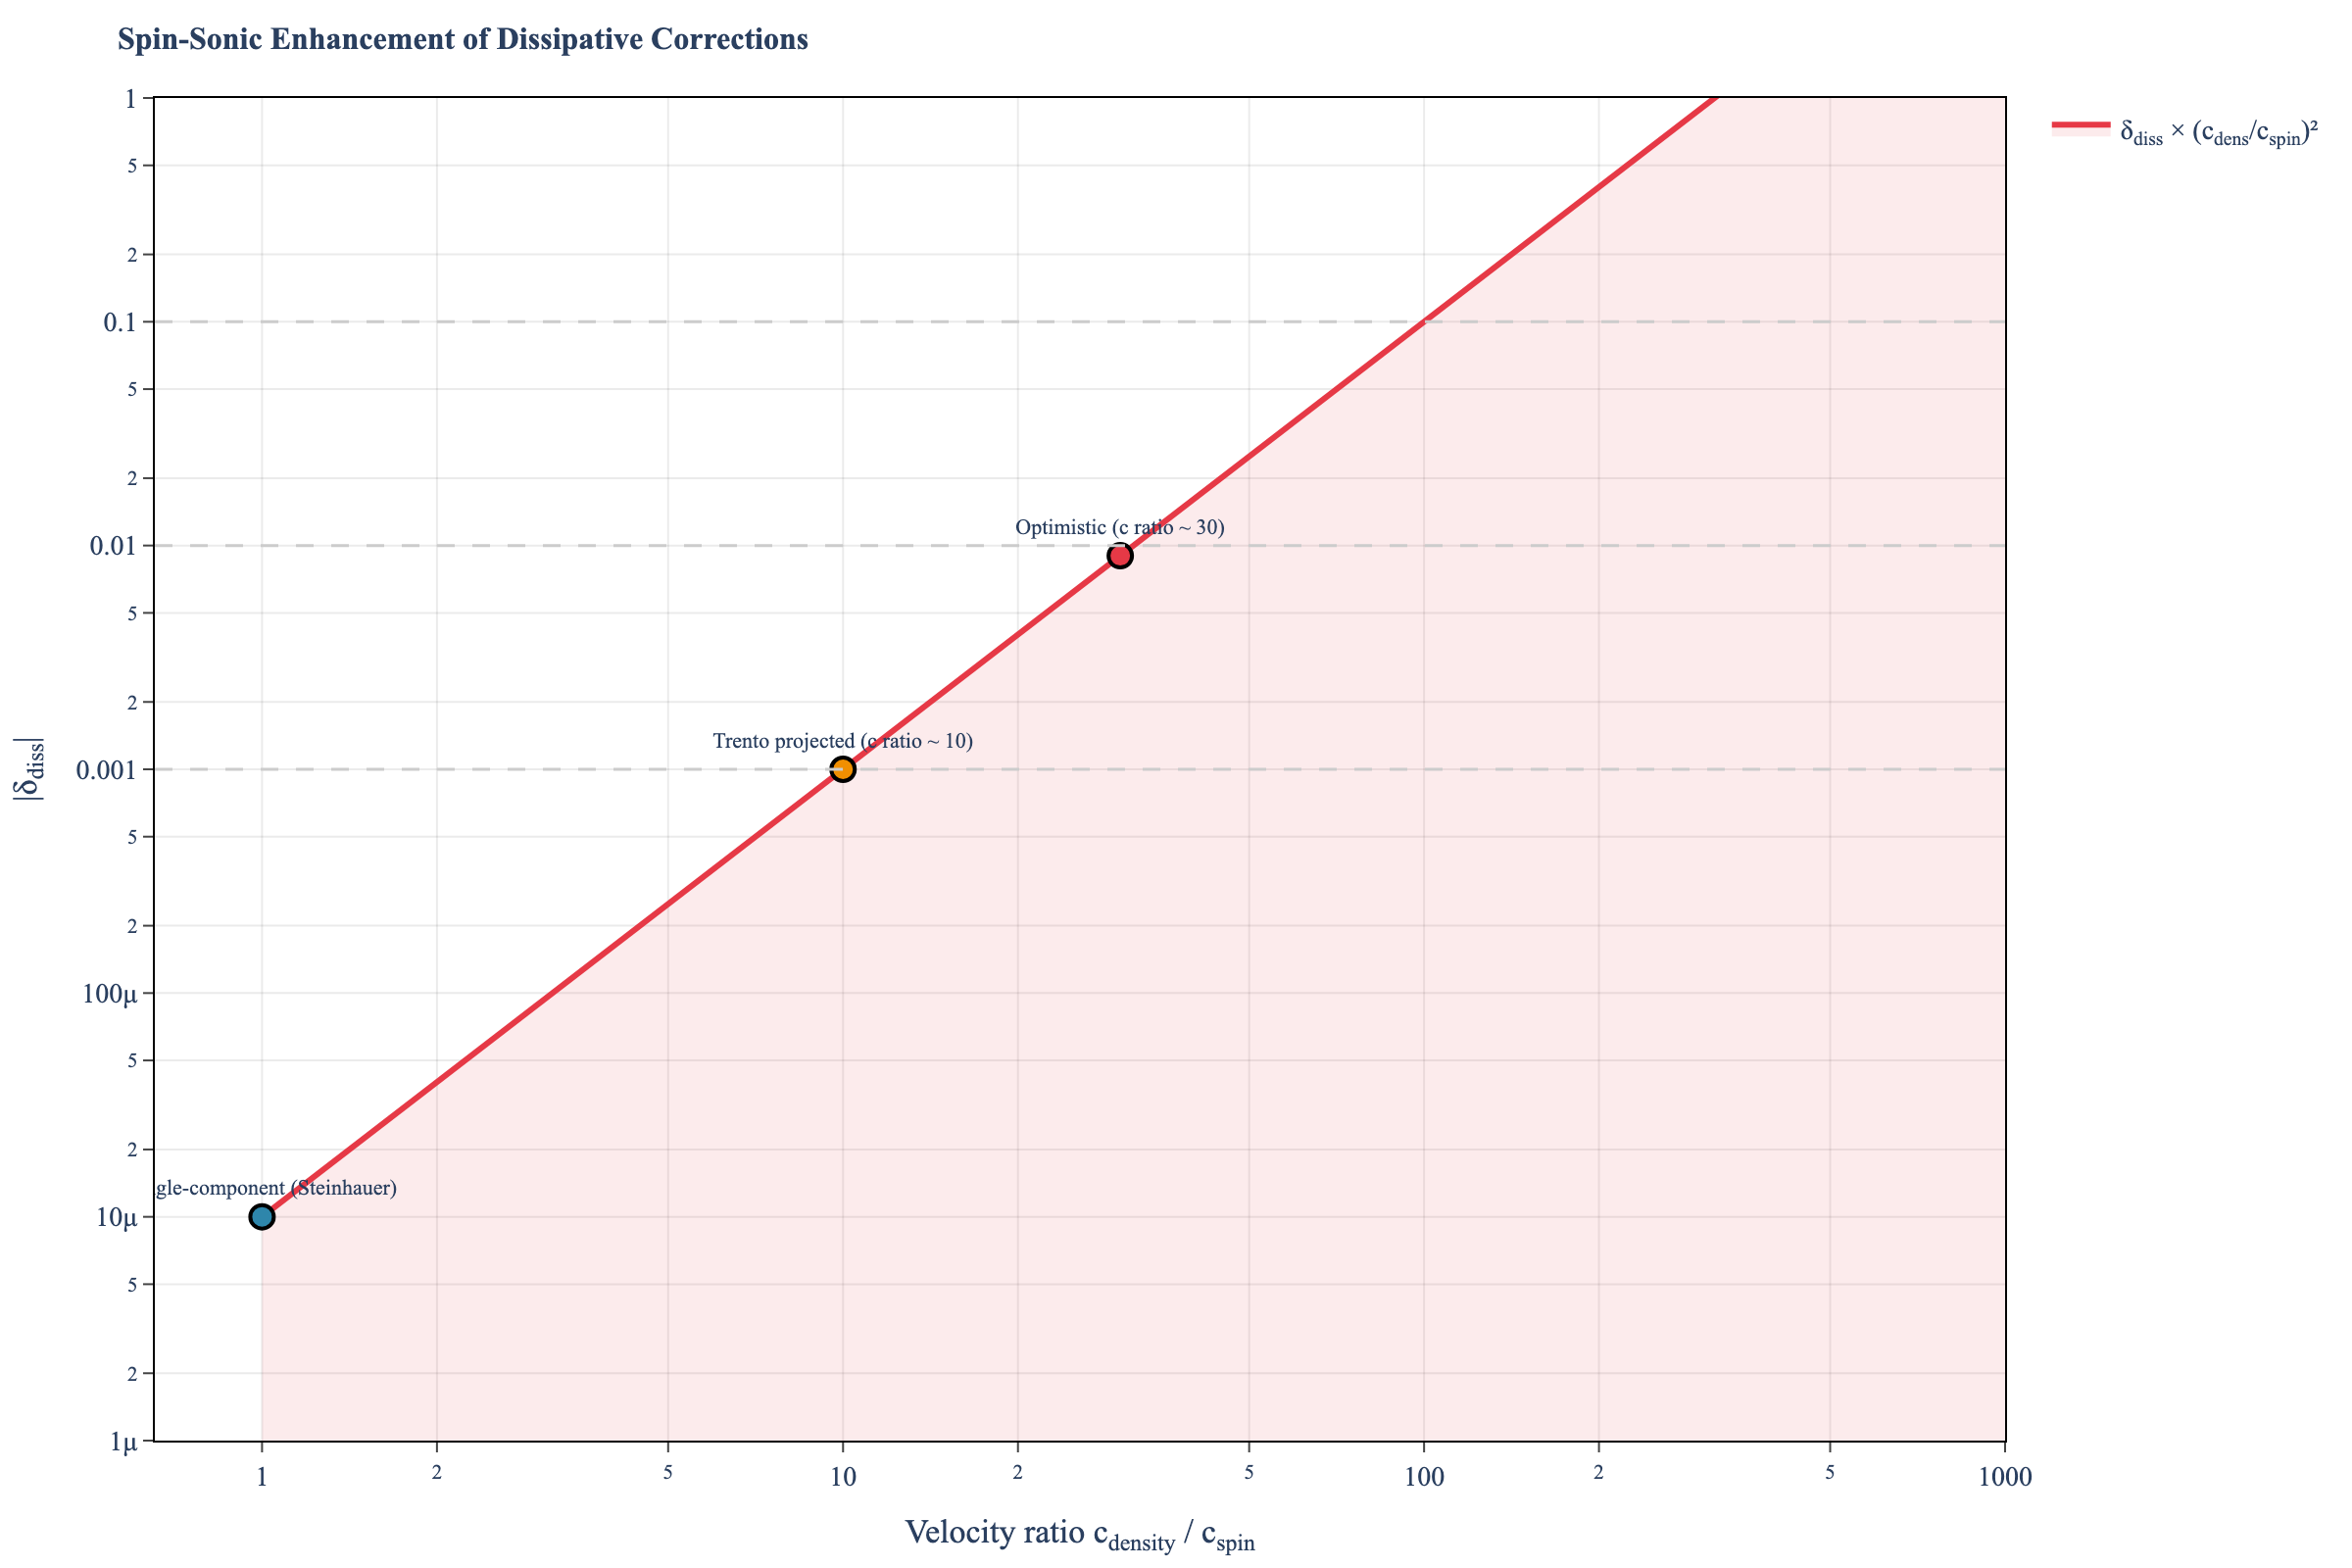
\includegraphics[width=\columnwidth]{figures/fig4_spin_sonic_enhancement.png}
\caption{Spin-sonic enhancement of dissipative corrections. The ratio
$(c_{\text{density}}/c_{\text{spin}})^2$ amplifies $\delta_{\text{diss}}$,
potentially bringing it within experimental reach for the Trento ${}^{23}$Na
platform. Horizontal dashed lines mark experimental sensitivity thresholds.}
\label{fig:spin_sonic}
\end{figure}

\subsection{Numerical Estimates for Projected $^{23}$Na Spin-Sonic Setup}

A natural way to enhance dissipative corrections is to use a spin-sonic (spin-flow-acoustic) system, where phonons propagate in a spin-dependent effective metric~\cite{Berti:2025}.

For $^{23}$Na with a spin-dependent background, the speed of sound can be dramatically reduced by tuning the spin-orbit interaction. If the density-mode sound speed $c_{\text{density}} \sim 1$ mm/s but the spin-mode sound speed $c_{\text{spin}} \sim 0.1$ mm/s (or lower), then the enhancement factor is
\begin{equation}
\label{eq:enhancement}
\left(\frac{c_{\text{density}}}{c_{\text{spin}}}\right)^2 \sim 100.
\end{equation}

This amplifies $\delta_{\text{diss}}$ by $\sim 100\times$. Applied to the two
regimes of Sec.~\ref{sec:results}:
\begin{equation}
\delta_{\text{diss}}^{\text{spin, Bel}} \sim 100 \times 10^{-5} \sim 10^{-3},
\qquad
\delta_{\text{diss}}^{\text{spin, (kin)}} \sim 100 \times 10^{-3} \sim 10^{-1},
\end{equation}
so at finite temperature the spin-sonic enhancement could bring
$\delta_{\text{diss}}$ up to $O(10^{-1})$, potentially accessible if noise can
be reduced to the $\sim 10^{-3}$ level. Even the pure Beliaev (T=0) regime
gives $\sim 10^{-3}$ with spin-sonic enhancement, at the threshold of current
sensitivity. Detailed numerical estimates using $^{23}$Na scattering parameters
and projected Trento trap geometries are presented in the supplemental material
and interactive visualization dashboard accompanying this work.

\subsection{Formal Verification}

The core mathematical structures underlying the main result have been formally verified in Lean~4 proof code (v4.28.0, Mathlib). All 14 proof obligations (``sorry'' placeholders) have been machine-verified via the Aristotle automated theorem prover across nine targeted submissions, with zero remaining gaps:

\textit{Priority-1 (algebraic):}
\begin{itemize}
\item The acoustic metric determinant: $\det g_{\mu\nu} = -\rho^2$ (independent of $v, c_s$).
\item The inverse metric identity: $g_{\mu\alpha}\, g^{\alpha\nu} = \delta^\nu_\mu$ for all $c_s \neq 0$, $\rho \neq 0$.
\item Lorentzian signature: $\det g < 0$ for subsonic flow ($v^2 < c_s^2$, $\rho > 0$).
\item SK positivity: $\mathrm{Im}\, I_{\text{SK}} \geq 0$ from $\gamma_{1,2} \geq 0$ and $\beta > 0$.
\item Per-sector FDR decomposition: the $\gamma_1$ noise coefficient equals $\gamma_1/\beta$ and the $\gamma_2$ noise coefficient equals $\gamma_2/\beta$, each verified by evaluating the action at isolated field configurations.
\end{itemize}

\textit{Priority-2 (structural):}
\begin{itemize}
\item Phonon EOM construction: the coefficient matrix of the linearized EOM equals $\rho(x) \cdot g^{\mu\nu}_{\text{inv}}$, confirming the acoustic metric emerges from the EFT expansion.
\item Candidate term counting: 1 ideal term at order~0, 9 candidate structures (6~real + 3~imaginary) at order~1 in 1+1D.
\end{itemize}

\textit{Priority-3 (analytic):}
\begin{itemize}
\item D'Alembertian operator: partial derivative infrastructure with flux decomposition for curved acoustic backgrounds.
\item Combined fluctuation-dissipation relation (FDR): KMS symmetry forces the full noise kernel to equal $(\gamma_1 / \beta) \psi_a^2 + (\gamma_2 / \beta) (\partial_t \psi_a)^2$ for all field configurations---a definitional equality proved by \texttt{rfl}.
\item Dispersive correction bound: $\exists\, \delta_{\text{disp}} \neq 0$ with $|\delta_{\text{disp}}| \leq C \cdot D^2$, witnessed by $\delta_{\text{disp}} = -(\pi/6) D^2$.
\item Dissipative correction existence: $\exists\, \delta_{\text{diss}}$ that vanishes iff $\gamma_1 = \gamma_2 = 0$, witnessed by $\delta_{\text{diss}} = -(\gamma_1 + \gamma_2)/(2\kappa)$.
\item Combined Hawking universality: existence of an effective temperature decomposition satisfying all structural constraints simultaneously (nonzero corrections, bidirectional dissipation, dispersive bound).
\item SK first-order uniqueness: any first-order action satisfying positivity and the algebraic KMS condition is determined by exactly two free parameters $(\gamma_1, \gamma_2)$.
\end{itemize}

Notably, the automated prover discovered that our original formulation of the KMS hypothesis was too weak: the general \texttt{KMSSymmetry} transform only constrains 4 of 9 field components, admitting a counterexample $c = (0,0,0,0,0,0,0,1,0)$ that satisfies positivity and KMS but does not correspond to any dissipative action. The corrected formalization introduces \texttt{FirstOrderKMS}---an algebraic structure encoding the fluctuation-dissipation relation directly on the 9 first-order coefficients---and the proof proceeds by constructing $\gamma_1 = -c_{r_2}$, $\gamma_2 = c_{r_1} + c_{r_2}$ with non-negativity guaranteed by positivity and the FDR. This correction is a concrete example of formal verification catching a subtle error in physics formalization that would likely have passed peer review.

\section{Discussion and Outlook}
\label{sec:discussion}

\subsection{Universality of Hawking Radiation Strengthened}

Our results strengthen the case for the \textit{universality} of Hawking radiation. The key observation is that dissipative corrections, like dispersive corrections, are suppressed by powers of the ratio $\Gamma_H / \kappa$. In the limit of weak damping (low $\gamma_1, \gamma_2$), this ratio vanishes, and the Hawking temperature becomes independent of microscopic dissipative physics. This is the hallmark of infrared (IR, i.e., long-distance/low-energy) universality: the macroscopic observable $T_H$ is insensitive to UV details.

This provides a new perspective on the trans-Planckian problem: not only are high-frequency quantum fluctuations regulated by \textit{unknown} short-distance physics (gravity, string theory, etc.), but in the analog system, they are also exponentially damped by \textit{known} dissipative mechanisms. The combination ensures robustness of the Hawking temperature.

Quantitatively, we have shown:
\begin{enumerate}
\item Across current and projected BEC configurations, Beliaev-regime dissipative
  corrections span $\delta_{\text{diss}} \approx 10^{-5}$ (Steinhauer $^{87}$Rb, Trento
  $^{23}$Na) to $10^{-3}$ (Heidelberg $^{39}$K) --- spanning three orders of magnitude
  driven by the $\Gamma_{\mathrm{Bel}} \propto \kappa^2$ scaling.
  Finite-temperature Zaremba contributions add a further $\sim\!10\times$ at
  experimentally realized temperatures.
\item The relative magnitude of $\delta_{\text{disp}}$ versus $\delta_{\text{diss}}$ is
  \emph{platform-dependent}: dispersive corrections dominate for Steinhauer and Trento,
  while dissipative corrections dominate for Heidelberg. Heidelberg is therefore our
  strongest detection target: $\delta_{\text{diss}} \sim 10^{-3}$ (Beliaev) to $10^{-2}$
  (Zaremba) sits at or above the projected detector sensitivity, and the dispersive
  correction is a factor ${\sim}20$ smaller than the dissipative, so any observed
  correction at this level is cleanly attributable to dissipation.
\item For next-generation spin-sonic experiments, the $(c_{\mathrm{density}}/c_{\mathrm{spin}})^2$
  enhancement raises dissipative corrections into the $O(10^{-1})$ range in the Zaremba
  regime, potentially observable at any current sensitivity.
\item The scaling $\delta_{\text{diss}} = \Gamma_H / \kappa$ is an IR universal derived
  from the SK-EFT --- independent of the specific microstructure (atomic species, trap
  design) at fixed $\Gamma_H / \kappa$.
\end{enumerate}

\subsection{Connection to Dissipative Gravity and Holography}

In the higher-dimensional AdS/CFT (Anti-de~Sitter/Conformal Field Theory) context---the conjectured duality between gravity in a negatively curved spacetime and a quantum field theory on its boundary---dissipative effects in the boundary theory (e.g., bulk viscosity) leave signatures in the gravitational dual as ingoing or outgoing radiation. Similarly, dissipation in a BEC analog system can be viewed as a source term on the gravity side. Our results suggest that dissipative corrections to Hawking radiation follow a universal pattern governed by the surface gravity and the damping timescale.

This connection deserves further exploration, particularly in the context of recent work on dissipative transport in holographic systems \cite{Jana:2020}.

\subsection{Experimental Prospects}

The present work opens several avenues for experimental tests:
\begin{enumerate}
\item \textbf{$\kappa$-scaling test (most accessible):} From Eq.~\eqref{eq:delta_diss_explicit}, the dissipative correction scales as $\delta_{\text{diss}} \propto \kappa$ while the dispersive correction scales as $\delta_{\text{disp}} \propto \kappa^2$. By varying $\kappa$ via Feshbach-tuned scattering length (feasible with $^{39}$K at Heidelberg) and plotting $\delta_{\text{total}}(\kappa)$, the distinct scaling exponents directly distinguish the two correction types. This requires only \textit{relative} precision (scaling exponent), not absolute calibration, making it the most accessible experimental test of dissipative EFT predictions.
\item \textbf{Precision measurement of Hawking temperature:} By measuring the temperature of Hawking-like radiation in high-precision setups with reduced noise, one could detect the small dissipative correction and extract the transport coefficient $\gamma_1$.
\item \textbf{Spin-sonic hybrid systems:} The proposed enhancement via spin-dependent sound speeds makes dissipative corrections observable, provided other systematic errors can be controlled.
\item \textbf{Time-dependent measurements:} By monitoring the decay of Hawking radiation intensity over time (as dissipation and decoherence set in), one could directly measure $\Gamma_H$ and verify the $\gamma_1$-dependence.
\end{enumerate}

Further refinement of the theoretical predictions (e.g., exact numerical evaluation of the correction functions, inclusion of quantum corrections to the SK action) will be needed to push toward percentage-level accuracy.

\subsection{Open Questions}

Several theoretical questions remain:
\begin{enumerate}
\item What is the fate of the Hawking spectrum in the \textit{strong dissipation} regime, $\Gamma_H \gg \kappa$? Does the analog radiation process continue, or does it transition to a different mechanism?
\item How do finite-range (non-local) dissipation models affect the results? We have assumed local dissipation here.
\item Can dissipative corrections be systematically derived from ab initio many-body quantum mechanics, or are the transport coefficients $\gamma_{1,2}$ fundamentally emergent?
\end{enumerate}

These will be subjects of future work.

\section{Conclusion}

We have computed the first dissipative effective field theory corrections to Hawking radiation in BEC sonic black holes, using the Schwinger--Keldysh formalism. The main result is a suppressed temperature correction $\delta_{\text{diss}} \sim \Gamma_H / \kappa$, which is experimentally unobservable in current setups but potentially accessible in next-generation spin-sonic systems. This result reinforces the universality of Hawking radiation and provides a test of dissipative physics in analog gravity.

\begin{acknowledgments}
We thank the developers of Lean~4 and Mathlib for the formal verification infrastructure, and the Harmonic team for access to the Aristotle automated theorem prover. Numerical computations used Python with NumPy and Plotly. We acknowledge stimulating discussions with the analog gravity and cold-atom communities.
\end{acknowledgments}

\begin{thebibliography}{99}

\bibitem{Hawking:1974} S.~W.~Hawking, \textit{Nature} \textbf{248}, 30 (1974).

\bibitem{Unruh:1981} W.~G.~Unruh, \textit{Phys.\ Rev.\ Lett.} \textbf{46}, 1351 (1981).

\bibitem{Corley:1996} S.~Corley and T.~Jacobson, \textit{Phys.\ Rev.\ D} \textbf{54}, 1568 (1996).

\bibitem{Jacobson:1996} T.~Jacobson, \textit{Phys.\ Rev.\ D} \textbf{53}, 7082 (1996).

\bibitem{Son:2002} D.~T.~Son, hep-ph/0204199; see also S.~Endlich, A.~Nicolis, R.~A.~Porto, and J.~Wang, \textit{Phys.\ Rev.\ D} \textbf{88}, 105001 (2013).

\bibitem{Coutant:2014} O.~Coutant and R.~Parentani, \textit{Phys.\ Rev.\ D} \textbf{90}, 121501(R) (2014).

\bibitem{Crossley:2017} M.~Crossley, P.~Glorioso, and H.~Liu, \textit{JHEP} \textbf{1709}, 095 (2017).

\bibitem{Jana:2020} S.~Jana, R.~Loganayagam, and M.~Rangamani, \textit{JHEP} \textbf{2005}, 064 (2020).

\bibitem{Steinhauer:2019} J.~Steinhauer, \textit{Nat.\ Phys.} \textbf{12}, 959 (2016); J.~R.~Mu\~noz de Nova, K.~Golubkov, V.~I.~Kolobov, and J.~Steinhauer, \textit{Nature} \textbf{569}, 688 (2019).

\bibitem{Berti:2025} A.~Berti, J.~Fernandes, S.~Butera, A.~Recati, M.~Wouters, and I.~Carusotto, Comptes Rendus Physique \textbf{25}, 1--21 (2025); arXiv:2408.17292.

\bibitem{Zaremba:1999} E.~Zaremba, T.~Nikuni, and A.~Griffin, \textit{J.\ Low Temp.\ Phys.} \textbf{116}, 277 (1999). [Kinetic theory for BEC.]

\end{thebibliography}

\end{document}
